\problem{ Gaz parfait de fermions non relativistes en deux dimensions}

\question{Calculez l'énergie de Fermi $\varepsilon_F$ en fonction de la densité $n = N/S$ du gaz.}

Pour un gas de fermion en 2D de spin $1/2$, le facteur de dégénérescence de spin est $g = 2$. 

L'énergie de Fermi est définie par la relation 
\[
    \varepsilon_F &= \frac{\hbar^2 k_F^2}{2m}, \label{eq: raw energy}
\]
où $k_F^2$ est le vecteur d'onde de Fermi.

De plus, en 2D, le potentiel chimique est défini tel que:
\[
    n &= \sum_{s} \int \frac{\dd^2k}{\qty(2\pi)^2} \Theta(\epsilon_F - \epsilon_{ks}) \notag \\
    \intertext{ce qui, pour un gaz non relativiste en 2D sans champ magnétique donne:}
    n &= \frac{gk_F^2}{4\pi} \notag \\
    &= \frac{gk_F^2}{4\pi}. \label{eq: deg spin}
\]

En isolant $k_F$ de l'équation (\ref{eq: deg spin}), on obtient:
\[
    k_F = \sqrt{2\pi n}.
\]

En substituant dans l'équation (\ref{eq: raw energy}) on trouve que l'énergie de Fermi est
\solution{energie fermi}{\epsilon_F = \frac{\hbar^2\pi n}{m}}

\question{Calculez l'énergie moyenne du gaz à température nulle.}

l'énergie moyenne d'un gaz par particule se trouve tel que
\[
    \expval{E} &= \frac{E}{N} \label{eq: la moyenne!}
\]
où $E$, l'énergie d'un gaz de Fermi en 2D et de spin $1/2$ est
\[
   E &= s\sum_s\int \frac{\dd^2k}{\qty(2\pi)^2} \epsilon{ks} \Theta(\epsilon_F - \epsilon_{ks}). \notag \\
   \intertext{Ce qui, pour un gaz non-relativiste en absence de champ magnétique donne}
   E &= \frac{s k_F^2}{2\pi} \notag \\
   &= \frac{1}{2}N\epsilon_F.
\]

En substituant l'équation précédente dans (\ref{eq: la moyenne!}) on obtient
\solution{energie moyenne}{\expval{E} = \frac{\epsilon_F}{2}}

\question{Calculez le potentiel chimique $\mu$ en fonction de $\varepsilon_F$ et de la température T.}

La densité moyenne d'un gaz en 2D est:
\[
    n &= \sum_s \int_0^\infty \frac{\dd^2k}{\qty(2\pi)^2} \frac{1}{e^{\beta\qty(\epsilon_{ks}-\mu)}+1}.
\]

En résolvant cette intégrale, on trouve 
\[
    n = \frac{m}{\pi\hbar^2} k_BT\ln\qty[1+e^{\frac{\mu}{kBT}}].
\]

Or, on a $\epsilon_F = \frac{\hbar^2\pi n}{m} \iff n = \frac{m}{\pi\hbar^2}$. 
En substituant dans l'équation précédente on trouve:
\[
    \epsilon_F &= k_BT\ln\qty[1+e^{\frac{\mu}{kBT}}] \notag
\]
d'où l'on peut isoler $\mu(T)$ pour obtenir

\solution{mu}{\mu(T) &= k_BT\ln(e^{\frac{\epsilon_F}{k_BT}}-1)}

En basse température, on a $T \ll T_F \Rightarrow e^{\frac{\epsilon_F}{k_BT}} \gg 1$.

On peut exprimer $\mu(T)$ tel que
\[
    \mu(T) &= \mu(T) &= k_BT\ln(e^{\frac{\epsilon_F}{k_BT}}-1) \notag \\
    &= \epsilon_F + k_BT\ln\qty(1 - e^{-\frac{\epsilon_F}{k_BT}}).
\]

Or, lorsque $T \ll T_F$, on a 
\[
    \ln\qty(1 - e^{-\frac{\epsilon_F}{k_BT}}) &\approx - e^{-\frac{\epsilon_F}{k_BT}} 
\]
d'où

\solution{basse temp}{\mu \approx \epsilon_F}

À haute température, on a $T \gg T_F$ d'où l'on peut trouver
\[
    e^{\frac{\epsilon_F}{k_BT}} -1 &\approx \frac{\epsilon_F}{k_BT}
\]
d'où l'on peut obtenir
\solution{haute temp}{k_BT\ln\qty(\frac{\epsilon_F}{k_BT})}

\begin{figure}[!ht]
        \centering
       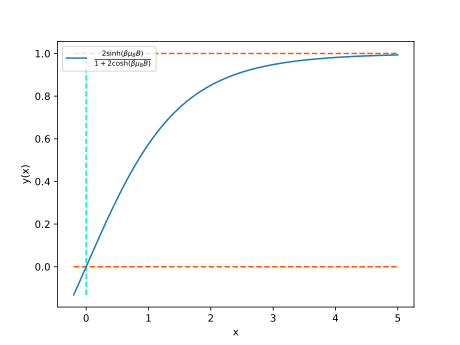
\includegraphics[scale= 0.8]{figs/no2v.PDF}
        \caption{$\mu(T)$}
        \label{fig: mu de t}
\end{figure}

Comme on peut l'observer sur la figure précédente, $\mu(T)$ change de signe à $T = T_F$.

\clearpage
